\chapter{Magic methods}
\section{Introduction}
Now that we have discussed both functions and classes, we can proceed to one of the features where Python really differs from e.g. JavaScript, namely the so called magic methods. These magic methods can be thought of as hooks, that allows the programmer to get to execute code at e.g. attribute access. We already showed in the section about classes how to handle the magic method \inlinecode{\_\_init\_\_}. This particular magic method is less interesting from many other magic methods, as it just corresponds to a constructor.

Two very important magic methods, however, are \inlinecode{\_\_getattribute\_\_} and \inlinecode{\_\_getattr\_\_}. These are particular interesting because each time an attribute \inlinecode{a} is read from a class object \inlinecode{x}, the following happens:

The magic method \inlinecode{\_\_getattribute\_\_} is looked up on \inlinecode{x}. If it is defined, the method is called with the instance, \inlinecode{x}, and the attribute name \inlinecode{a}. It is now up to the supplied method to return the correct value\inlinecode{For instance the implementation of \inlinecode{\_\_getattribute\_\_} could just return a constant, which would cause every attribute access to result in that particular constant.}. If the implementation of \inlinecode{\_\_getattribute\_\_} happens to raise an \inlinecode{AttributeError}, \inlinecode{\_\_getattr\_\_} is called. Otherwise if \inlinecode{\_\_getattribute\_\_} is not defined, the attribute is looked up on the instance. If the attribute is present on the instance it is returned, otherwise an \inlinecode{AttributeError} is raised and the magic method \inlinecode{\_\_getattr\_\_} is called (at least if it is defined).

The following pseudo code should illustrate this:

\begin{listing}[H]
	\begin{minted}[linenos]{python}
def readAttribute(x, a):
  __getattribute__ = lookup(x, '__getattribute__')
  __getattr__ = lookup(x, '__getattr__')

  try:
    if isset(__getattribute__):
      # __getattribute__ is called if defined
      return __getattribute__(x, a)
    else:
      return getattr(x, a)
  except AttributeError as e:
    if isset(__getattr__):
      # __getattr__ called in case of an AttributeError
      return __getattr__(x, a)
    else
      raise e
	\end{minted}
\end{listing}

Thus, the magic method \inlinecode{\_\_getattribute\_\_} can be used to supply a custom attribute lookup function, and \inlinecode{\_\_getattr\_\_} can be used to supply a fallback function in case of a bad attribute access. Note also that the \inlinecode{\_\_getattribute\_\_} can not be thought of as being equivalent (or nearly equivalent) to getters in e.g. ECMAScript 5 and C\#: In Python one single method is supplied, not one for each attribute (or property and field for ECMAScript 5, respectively C\#).

As mentioned in the introduction we have only aimed to support \inlinecode{\_\_getattr\_\_} in our type analyzer, due to the limited time of our project. However, in order to determine that we wanted to support \inlinecode{\_\_getattr\_\_} and not \inlinecode{\_\_getattribute\_\_}, we looked at the use of these magic methods in some larger Python projects. In Django 1.5.1\footnote{See \url{http://www.djangoproject.com/}.}, a high-level web framework, we found that \inlinecode{\_\_getattribute\_\_} was not used at all. However, \inlinecode{\_\_getattr\_\_} is used 14 times and therefore seems more useful to support if the choice stands between the two of them. Of course 14 usages is not much for a web framework on approximately 200.000 lines of code, but it is still essential to handle in order to be able to statically analyze Python programs.

\section{Transforming the CFG}
Since each single attribute access possibly involves method calls, we normalize the CFG in order to reflect this. More concretely, we normalize each node in the CFG of the following form: \inlinecode{<res>=ReadAttribute(<base>,prop)}, into the following CFG piece:

\begin{listing}[H]
	\begin{center}
		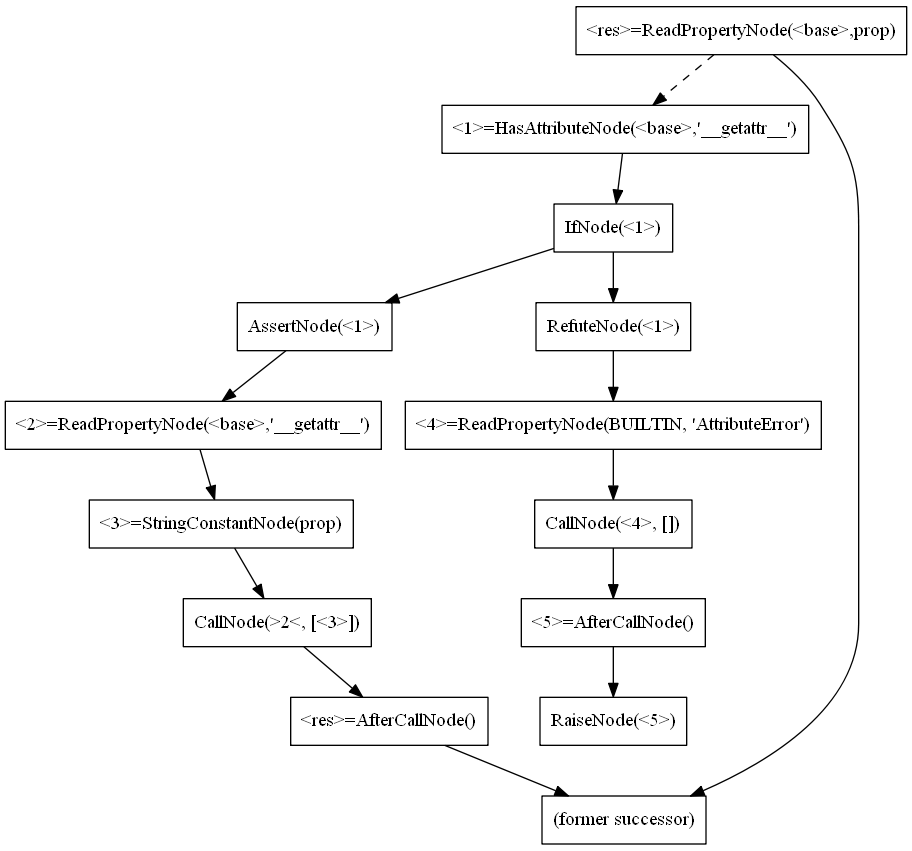
\includegraphics[width=0.9\textwidth]{images/readproperty.png}
	\end{center}
	\vspace{-10pt}
	\caption{The normalization of a read attribute node.}
	\label{fig:MagicMethods1}
\end{listing}

As can be seen from the normalized CFG of read attribute nodes the only challenge there is in order for our analysis to handle the magic method \inlinecode{\_\_getattr\_\_}, is that we need to handle exceptions in our analysis. We return to this in the following section. First, we want to note that if an attribute is \textit{definately} set on an instance object, \inlinecode{\_\_getattr\_\_} is never called when reading that particular attribute. This is the case as there won't be any flow across the exception edge in the figure above, because the \inlinecode{ReadAttributeNode} will always succeed in reading the attribute and therefore not raise any \inlinecode{AttributeError}. When we can't conclude that an attribute is definately available (e.g. as in the example below), we must of course normalize the read attribute node.

\begin{listing}[H]
	\begin{minted}[linenos]{python}
class C():
  if (trickyComputation()):
    C.a = 42
  def __getattr__(self, name):
    return "<bad attribute access>"
x = C()
y = x.a # __getattr__ will be called if trickyComputation() returned false
	\end{minted}
	\caption{A simple example of when it will be possible to conclude that \inlinecode{\_\_getattr\_\_} will never be called even though \inlinecode{\_\_getattribute\_\_} is defined.}
	\label{code:MagicMethods2}
\end{listing}

Thus the type analyzer can be improved such that it only normalizes read attribute nodes if the attribute being read may not be defined (resulting in possibly $12 * \#\texttt{read attribute nodes}$ nodes less in the CFG). This is in fact what our implementation does. In order to obtain this we have provided the analysis with a hook from the worklist algorithm, such that our type analyzer can modify the control flow graph during the analysis. When doing this, each newly added node to the CFG must of course be added to the worklist.

It is important to note however, that not supporting \inlinecode{\_\_getattribute\_\_} simplifies the task a bit. Recall that we don't need to normalize read attribute nodes as long the attribute being read is definately set. This is not the case if we took the magic method \inlinecode{\_\_getattribute\_\_} into account, as it might itself raise an \inlinecode{AttributeError} (causing \inlinecode{\_\_getattr\_\_} to be called)! Thus a type analysis that also supports \inlinecode{\_\_getattribute\_\_} would for a start actually have to normalize all read attribute nodes where an attribute is dereferenced from an instance that belongs from a class where \inlinecode{\_\_getattribute\_\_} is defined. In some cases it might of course be possible to conclude that the particular implementation of \inlinecode{\_\_getattribute\_\_} will never raise an \inlinecode{AttributeError}, e.g. when the implementation just returns a constant (see the example below), in which the type analysis of course don't need to normalize the read property node.

\begin{listing}[H]
	\begin{minted}[linenos]{python}
class C(object):
  def __getattribute__(self, name):
    return 42
  def __getattr__(self, name):
    return "<bad attribute access>"
x = C()
y = x.a # no attribute access will result in __getattr__ being called
	\end{minted}
	\caption{A simple example of when it will be possible to conclude that \inlinecode{\_\_getattr\_\_} will never be called even though \inlinecode{\_\_getattribute\_\_} is defined.}
	\label{code:MagicMethods2}
\end{listing}